\documentclass[]{article}

\title{FSS Simulation Toolkit v0.1 \\ User's Guide}
\author{Paul T. Grogan\footnote{ptgrogan@mit.edu}}
\date{Revised \today}

\usepackage[backend=bibtex,style=authoryear,sorting=nyt,firstinits=true,maxnames=2,maxbibnames=99]{biblatex}
\addbibresource{bibtex.bib}

% http://tex.stackexchange.com/questions/126226/how-do-i-instruct-fullcite-to-use-maxbibnames-rather-than-maxcitenames
\makeatletter
\DeclareCiteCommand{\fullcite}
  {\defcounter{maxnames}{\blx@maxbibnames}%
    \usebibmacro{prenote}}
  {\usedriver
     {\DeclareNameAlias{sortname}{default}}
     {\thefield{entrytype}}}
  {\multicitedelim}
  {\usebibmacro{postnote}}
\DeclareCiteCommand{\footfullcite}[\mkbibfootnote]
  {\defcounter{maxnames}{\blx@maxbibnames}%
    \usebibmacro{prenote}}
  {\usedriver
     {\DeclareNameAlias{sortname}{default}}
     {\thefield{entrytype}}}
  {\multicitedelim}
  {\usebibmacro{postnote}}
\makeatother

\usepackage{url}
\usepackage{dirtree}
\usepackage{import}
\usepackage{graphicx}
\graphicspath{{img/}}
\DeclareGraphicsExtensions{.png}

\usepackage{tikz}
\usepackage[simplified]{pgf-umlcd}

\usepackage[margin=1.25in]{geometry}

%http://stackoverflow.com/questions/3175105/how-to-insert-code-into-a-latex-doc/3175141#3175141
\usepackage{listings}
\definecolor{dkgreen}{rgb}{0,0.6,0}
\definecolor{gray}{rgb}{0.5,0.5,0.5}
\definecolor{mauve}{rgb}{0.58,0,0.82}
\lstset{frame=tblr,
  language=Java,
  showstringspaces=false,
  columns=flexible,
  basicstyle={\small\ttfamily},
  numbers=left,
  numberstyle=\tiny\color{gray},
  keywordstyle=\color{blue},
  commentstyle=\color{dkgreen},
  stringstyle=\color{mauve},
  breaklines=true,
  breakatwhitespace=true,
  tabsize=4
}
\renewcommand\lstlistingname{Box}

% http://tex.stackexchange.com/questions/10141/how-to-prevent-lstlisting-from-splitting-code-between-pages
\usepackage{float}
\floatstyle{plain}
\newfloat{Code}{H}{myc}

\usepackage{verbatim}

\begin{document}
\maketitle

\section{Introduction}

This user's guide covers the FSS Simulation Toolkit (the ``toolkit'') which was developed during academic year 2013-4 as a part of the Federated Satellite Systems (FSS) joint project between the Massachusetts Institute of Technology and Skolkovo Institute of Technology (P.I. Prof. de Weck and Co-P.I. Prof. Golkar). This document extends high-level discussion of the toolkit developed and used in support in the initial conference paper:
\begin{quote}
\small
\fullcite{grogan13}
\end{quote}
to include installation and configuration notes and extended discussion of examples and tutorials. The intent is to eventually release the toolkit as an open source library under a permissive license at which time this document should be transformed to a community-accessible format such as a wiki.

As discussed in the above conference paper, a FSS is a system-of-systems (SoS) of constituent spacecraft exhibiting resource exchanging behaviors. Each FSS member voluntarily joins out of mutual benefit and no centralized authority can exert control the total SoS. An isomorphic simulation architecture, i.e. one which provides decentralized control over member simulation models, is desired to aid design activities. For example, it may be used to formulate mechanisms for service provision under partial information, to identify integration requirements between FSS members, or simply to distribute conceptual spacecraft designs among various teams.

This toolkit is based on an existing standard for interoperable simulation called the High Level Architecture (HLA, IEEE Standard 1516-2010). The HLA defines the interface between a member simulation model (a ``federate'') and rest of the SoS simulation (a ``federation''). It relies on a runtime implementation (RTI) to manage key processes such as federation, data, object, and time management. As a mature standard, there are several RTI implementations available, both commercially licensed and open source with permissive licensing.

The HLA is an interoperability standard which minimizes assumptions of the detailed implementation of federates. RTI implementations, however, generally only support mature high-level languages such as Java, C, and C++. Based on the development experience of this author and on the wide availability of open source libraries with permissive licensing, Java was selected as the toolkit's implementation language. Other languages could be supported under a FSS federation; however they must be supported by a selected RTI and ports of this toolkit would be necessary to conform to the expected federation object model (FOM) and federation agreement discussed in \textcite{grogan13}.

Figure \ref{fig:federationArchitecture} illustrates the overall structure of a HLA federation. The independent federates ($\alpha$, $\beta$, and $\gamma$) communicate with each other according to standard services via the RTI. Data structures within messages are based on the common form specified in the FOM. The particular method of communication is not specified by the HLA standard. Instead, each federate uses a federate ambassador to receive information from the rest of the federation and accesses an RTI ambassador to send information to the federation.

\begin{figure}
\centering
\small
\import{img/}{federationArchitecture.pdf_tex}
\caption{Structure of an HLA federation. Federates receive information via a federate amabssador and send information via an RTI ambassador.}
\label{fig:federationArchitecture}
\end{figure}

\section{Toolkit Installation and Configuration}

This section describes how to download and configure the toolkit to run the example federates. 
\subsection{Installation}

As of this time there is no installer script for the toolkit. Instead, it is used within an integrated development environment (IDE) to help manage dependent libraries. There are several excellent Java IDEs which could alternatively be used to develop applications using the toolkit, however this author is most familiar with Eclipse.

\begin{enumerate}
\item Download and install the Eclipse IDE:
\begin{enumerate}
\item Download the Eclipse IDE for Java: \\ \url{http://www.eclipse.org/downloads/packages/eclipse-ide-java-developers/}
\item Extract the .zip file to a desired file location (there is no installer).
\item Run the \texttt{eclipse.exe} executable and choose a local workspace location.
\end{enumerate}
\item Install the Subclipse extension for integrated SVN access:
\begin{enumerate}
\item Select ``Help $>$ Eclipse Marketplace...'' from the Eclipse menu.
\item Search for ``Subclipse'' and click ``Install'' for a match (version Subclipse 1.10.3 as of writing).
\item Select all features, click ``Confirm,'' and accept the license agreement to install.
\item Restart Eclipse to complete installation.
\end{enumerate}
\item Checkout the FSS toolkit:
\begin{enumerate}
\item Select ``File $>$ New $>$ Other'' from the Eclipse menu.
\item Expand the ``SVN'' folder, select ``Checkout Projects from SVN'' and click ``Next'' to continue.
\item Select ``Create a new repository location'' and click ``Next'' to continue.
\item Enter the URL \url{svn://ptgrogan.scripts.mit.edu/fss/} and click ``Next'' to continue.
\item Select the \texttt{trunk} directory and click ``Finish'' to continue.
\item Expand the ``Java'' folder, select ``Java Project'' and click ``Next'' to continue.
\item Give the project a name, change other options (if desired, note: Java SE 7 is the minimum version required), and click ``Finish'' to download the source files.
\end{enumerate}
\item Configure the FSS toolkit in Eclipse:
\begin{enumerate}
\item Select ``Project $>$ Properties'' from the Eclipse menu, select the ``Java Build Path'' item from the left-hand menu, and select the ``Libraries'' tab on the right.
\item Click the ``Add JARs...'' button and select the following:
\begin{enumerate}
\item \texttt{lib/commons-math3-3.2/commons-math3-3.2.jar}
\item \texttt{lib/jfreechart-1.0.17/jcommon-1.0.21.jar}
\item \texttt{lib/jfreechart-1.0.17/jfreechart-1.0.17.jar}
\item \texttt{lib/log4j-1.2.17/log4j-1.2.17.jar}
\item \texttt{lib/ohla-0.6/ohla-0.6.jar}
\item \texttt{lib/orekit-6.0/orekit-6.0.jar}
\item \texttt{lib/portico-2.0.0/portico.jar}
\item \texttt{lib/worldwind-2.0-857.1737/worldwind.jar}
\end{enumerate}
\item Click ``OK'' to add the JARs to the project library.
\item \textbf{Optionally} expand JAR files, select the Javadoc location item, click ``Edit...,'' and select the appropriate Javadoc file to provide documentation within the Eclipse IDE:
\begin{enumerate}
\item Commons Math 3: Javadoc in archive, Workspace file: \\ \texttt{lib/commons-math3-3.2/commons-math3-3.2-javadoc.jar}
\item JFreeChart: Javadoc in archive, Workspace file: \\ \texttt{lib/jfreechart-1.0.17/jfreechart-1.0.17-javadocs.zip}
\item Log4J: Javadoc in archive, Workspace file: \\ \texttt{lib/log4j-1.2.17/log4j-1.2.17-apidocs.zip}
\item Orekit: Javadoc in archive, Workspace file: \\ \texttt{lib/orekit-6.0/orekit-6.0-javadoc.jar}
\item World Wind: Javadoc in archive, Workspace file: \\ \texttt{lib/worldwind-2.0-857.1737/worldwind-docs-daily-857.1737.zip}
\end{enumerate}
\item Click ``OK'' to close the project properties. The project should re-build automatically and all errors should disappear.
\end{enumerate}
\item Test the example federates:
\begin{enumerate}
\item Select the CosmosSkyMED-1 example federate in the file tree \\ \texttt{edu.mit.fss.examples/CosmoSkyMed1.java} and click the green ``Run'' button in Eclipse.
\item Click the plug icon, then click the play icon in the GUI to initialize the federate and start advancing time.
\item Select the Visualization example federate in the file tree \\ \texttt{edu.mit.fss.examples/Visualization.java} and click the green ``Run'' button in Eclipse.
\item Click the plug icon in the visualization federate GUI; it should halt the federation execution. (Note: if the federates were run in the reverse order, CosmosSkyMED-1 would wait for the time to reach October 2013 before halting the federation.)
\item Click the play icon in the visualization federate GUI; it should allow time to advance in both federates.
\end{enumerate}
\end{enumerate}

\subsection{Network Configuration}

Any number of federates can be run on a single computer through the default loop-back interface, but to enable distributed simulation of federates across multiple computers each participant must be connected to a network and configured. There are two different configurations depending on if the Portico or OHLA runtime infrastructures (RTIs) are used.

\subsubsection{Portico RTI}

The Portico RTI is a decentralized implementation where each federate uses a local RTI component (LRC) with no central RTI component (CRC). Communication uses a UDP multi-cast protocol which may be blocked by shared network infrastructure. Due to these limitations, a local area network (LAN) with a private router may be required to host a distributed simulation.

\begin{enumerate}
\item Connect each participant to the local network (wired or wireless).
\item If there are multiple network interfaces, select the correct bind address for Portico by configuring the \texttt{portico.jgroups.udp.bindAddress} property in the \texttt{RTI.rid} file (uncomment and add the IP address on the private LAN).
\item Depending on security settings, software firewalls (i.e. Windows Firewall) may need to be disabled or have new rules added to allow UDP traffic.
\end{enumerate}

\subsubsection{OHLA RTI}

The OHLA RTI uses a centralized implementation where each federate uses a local RTI component (LRC) which connects with a central RTI component (CRC) running separately. Communication uses a common TCP protocol which is generally supported over wide area networks (WANs). 

\begin{enumerate}
\item Connect each participant to the network (wired or wireless).
\item Select the desired CRC port (default 15000) by associated property in the \texttt{ohla-crc.properties} file and start the CRC program.
\item Select the corresponding CRC host (default 127.0.0.1) and port (default 15000) by changing the associated properties in the \texttt{ohla-lrc.properties} file.
\item Depending on security settings, software firewalls (i.e. Windows Firewall) may need to be disabled or have new rules added to allow TCP traffic on the desired port.
\end{enumerate}

\section{Toolkit Contents}

The toolkit is presently stored in a Subversion repository hosted by the M.I.T. Scripts service. Its files and history is publicly-accessible at the URL:
\begin{center}
\url{svn://ptgrogan.scripts.mit.edu/fss/}
\end{center}
This repository is set to anonymous read access and authenticated write access. While anyone can download the files, only authorized developers can make changes. Future development may migrate to an open source repository service to more easily allow community contributions.

The repository contains the following directory structure:
\dirtree{%
.1 svn://ptgrogan.scripts.mit.edu/fss/.
.2 branches/.
.2 tags/.
.2 trunk/.
.3 src/.
.4 edu.mit.fss.
.4 edu.mit.fss.event.
.4 edu.mit.fss.examples.
.4 edu.mit.fss.hla.
.4 edu.mit.fss.tutorial.
.4 resources.
.3 doc/.
.3 lib/.
.3 lib-external/.
.3 license.txt.
}
The root \texttt{trunk/} directory contains several configuration and data files. The \texttt{src/} directory contains the source code within the \texttt{edu.mit.fss} package structure and icons in the \texttt{resources} package. The \texttt{doc/} directory contains documentation including this user guide. The \texttt{lib/} and \texttt{lib-external/} directories contain redistributable third-party libraries. Finally, the \texttt{license.txt} file contains the standard 2-clause BSD license under which the toolkit is released.

\subsection{Core Toolkit Interfaces}

The core toolkit interfaces provide the top-level structure and require methods for Java object classes participating in a FSS simulation. The following files define the core interfaces to the FSS simulation toolkit:
\dirtree{%
.1 trunk/.
.2 src/.
.3 edu.mit.fss.
.4 Element.java\DTcomment{Interface to an element with Cartesian coordinates}.
.4 OrbitalElement.java\DTcomment{Interface to an element with Keplerian orbital elements}.
.4 Receiver.java\DTcomment{Interface to a RCP receiver abstraction}.
.4 ReferenceFrame.java\DTcomment{Enumeration of existing reference frames}.
.4 Signal.java\DTcomment{Interface to a RCP signal abstraction}.
.4 SimInteraction.java\DTcomment{Interface to a simulation interaction}.
.4 SimObject.java\DTcomment{Interface to a simulation object}.
.4 SurfaceElement.java\DTcomment{Interface to an element with geodetic coordinates}.
.4 Transmitter.java\DTcomment{Interface to a RCP transmitter abstraction}.
}
Figure \ref{fig:coreInterfaceOCD} illustrates an object class diagram of the core interface classes. A few classes introduce external dependencies. First, the \texttt{Vector3D} data type used in the \texttt{Element} type is from the Apache Commons Math 3 library. Second, the \texttt{Frame} data type used in the \texttt{ReferenceFrame} enumeration is from the Orekit flight dynamics library.

\begin{figure}
\centering
\footnotesize
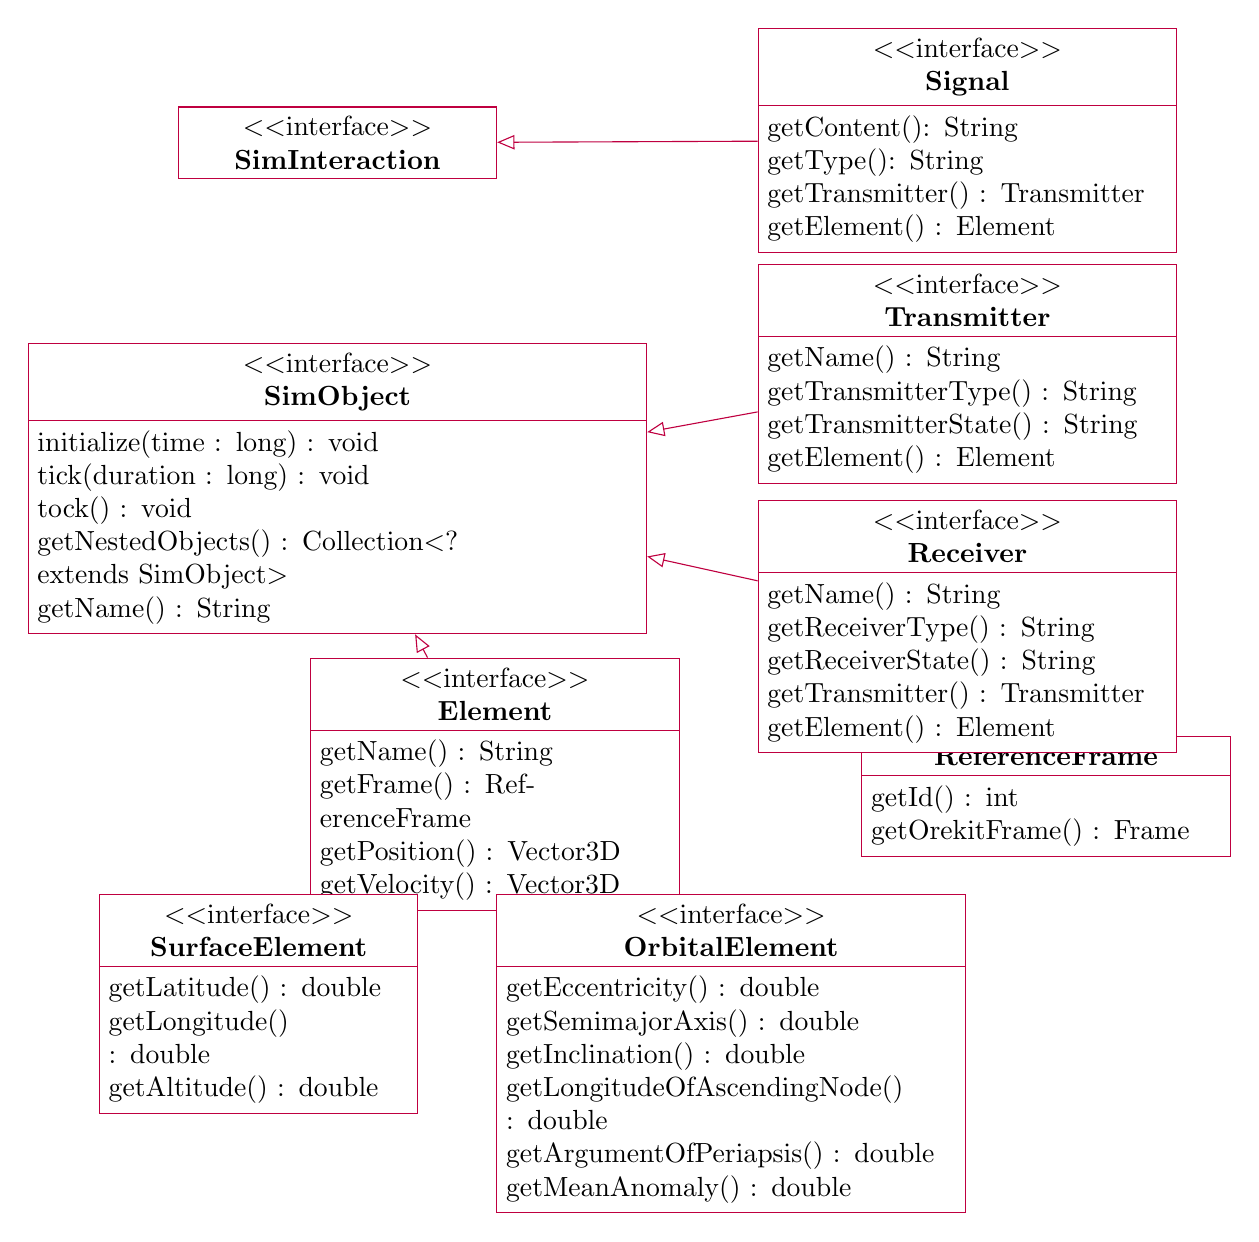
\begin{tikzpicture}% [ show background grid ]
\begin{interface}[text width=3in,fill=white]{SimObject}{-4,4}
\operation{initialize(time : long) : void }
\operation{tick(duration : long) : void }
\operation{tock() : void }
\operation{getNestedObjects() : Collection$<$? extends SimObject$>$ }
\operation{getName() : String }
\end{interface}

\begin{interface}[text width=1.5in,fill=white]{SimInteraction}{-4,7}
\end{interface}

\begin{interface}[text width=1.75in,fill=white]{Element}{-2,0}
\inherit{SimObject}
\operation{getName() : String }
\operation{getFrame() : ReferenceFrame }
\operation{getPosition() : Vector3D }
\operation{getVelocity() : Vector3D }
\end{interface}

\begin{class}[text width=1.75in,fill=white]{ReferenceFrame}{5,-1}
\operation{getId() : int }
\operation{getOrekitFrame() : Frame }
\end{class}
%\composition{Element}{}{}{ReferenceFrame}

\begin{interface}[text width=1.5in,fill=white]{SurfaceElement}{-5,-3}
\inherit{Element}
\operation{getLatitude() : double }
\operation{getLongitude() : double }
\operation{getAltitude() : double }
\end{interface}

\begin{interface}[text width=2.25in,fill=white]{OrbitalElement}{1,-3}
\inherit{Element}
\operation{getEccentricity() : double }
\operation{getSemimajorAxis() : double }
\operation{getInclination() : double }
\operation{getLongitudeOfAscendingNode() : double }
\operation{getArgumentOfPeriapsis() : double }
\operation{getMeanAnomaly() : double }
\end{interface}

\begin{interface}[text width=2in,fill=white]{Transmitter}{4,5}
\inherit{SimObject}
\operation{getName() : String }
\operation{getTransmitterType() : String }
\operation{getTransmitterState() : String }
\operation{getElement() : Element}
\end{interface}

\begin{interface}[text width=2in,fill=white]{Receiver}{4,2}
\inherit{SimObject}
\operation{getName() : String }
\operation{getReceiverType() : String }
\operation{getReceiverState() : String }
\operation{getTransmitter() : Transmitter}
\operation{getElement() : Element}
\end{interface}

\begin{interface}[text width=2in,fill=white]{Signal}{4,8}
\inherit{SimInteraction}
\operation{getContent(): String}
\operation{getType(): String}
\operation{getTransmitter() : Transmitter}
\operation{getElement() : Element}
\end{interface}
\end{tikzpicture}
\caption{Object class diagram of the FSS simulation toolkit core interfaces}
\label{fig:coreInterfaceOCD}
\end{figure}

\subsection{HLA Model Implementations}

The HLA model implementations use the core interfaces to define objects compatible with the HLA runtime infrastructure (RTI). For example, a ``remote'' object in a federation will appear as a HLA model implementation, as will a copy of a ``local'' object to facilitate information exchange with the federation. The following classes implement the core interfaces using HLA data types:
\dirtree{%
.1 trunk/.
.2 src/.
.3 edu.mit.fss.hla.
.4 FSScartesianVector.java\DTcomment{HLA implementation of \texttt{Vector3D} type}.
.4 FSSelement.java\DTcomment{HLA implementation of \texttt{Element} interface}.
.4 FSSorbitalElement.java\DTcomment{HLA implementation of \texttt{OrbitalElement} interface}.
.4 FSSreceiver.java\DTcomment{HLA implementation of \texttt{Receiver} interface}.
.4 FSSreferenceFrame.java\DTcomment{HLA implementation of \texttt{ReferenceFrame} type}.
.4 FSSsignal.java\DTcomment{HLA implementation of \texttt{Signal} interface}.
.4 FSSsurfaceElement.java\DTcomment{HLA implementation of \texttt{SurfaceElement} interface}.
.4 FSStransmitter.java\DTcomment{HLA implementation of \texttt{Transmitter} interface}.
.4 HLAinteraction.java\DTcomment{HLA helper class for managing interactions}.
.4 HLAobject.java\DTcomment{HLA helper class for managing objects}.
.4 OHLA\_CRC.java\DTcomment{Main method to start OHLA central RTI component}.
}
The helper class implementations \texttt{HLAinteraction} and \texttt{HLAobject} work with the federate ambassador to send and receive updates automatically from the federation. Figure \ref{fig:hlaImplementationOCD} illustrates a simplified object class diagram of the HLA model implementation classes.

\begin{figure}
\centering
\footnotesize
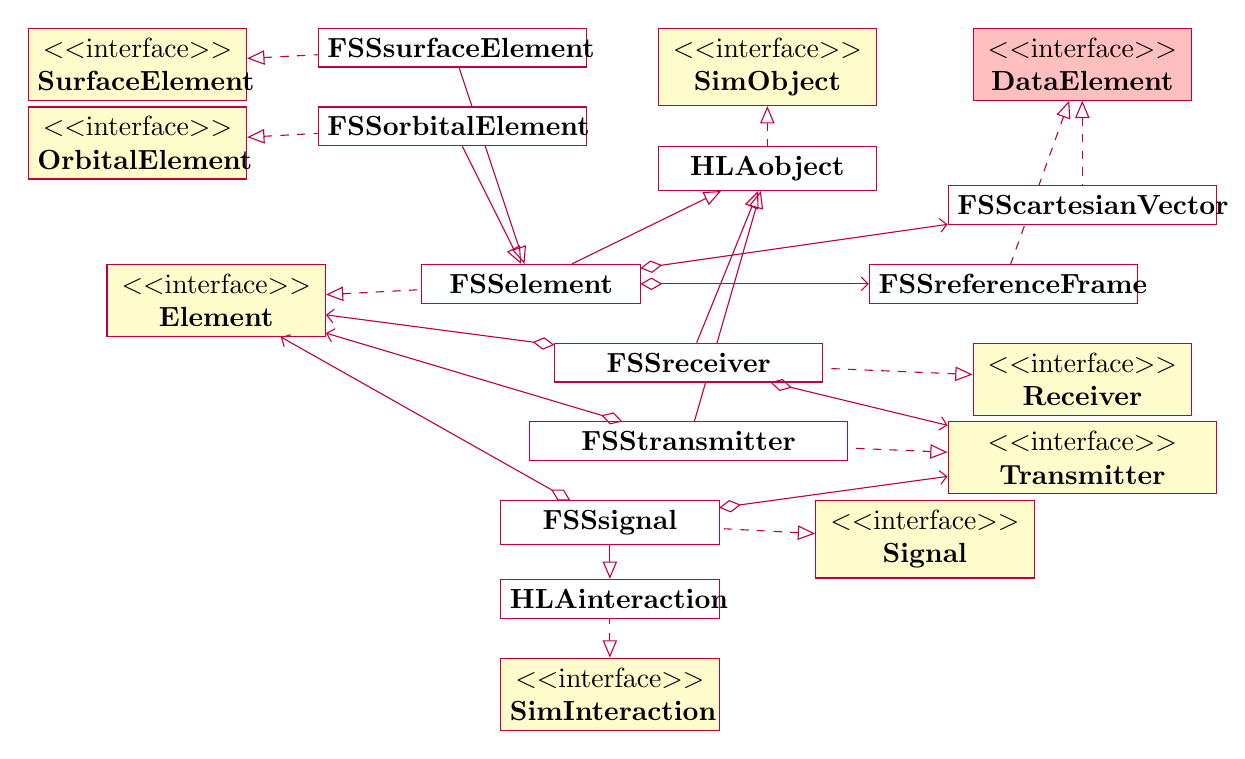
\begin{tikzpicture}% [ show background grid ]
\begin{interface}[text width=1in,fill=pink]{DataElement}{4,2}
\end{interface}

\begin{class}[text width=1.25in,fill=white]{FSScartesianVector}{4,0}
\implement{DataElement}
\end{class}

\begin{class}[text width=1.25in,fill=white]{FSSreferenceFrame}{3,-1}
\implement{DataElement}
\end{class}

\begin{interface}[text width=1in]{SimObject}{0,2}
\end{interface}


\begin{class}[text width=1in,fill=white]{HLAobject}{0,.5}
\implement{SimObject}
\end{class}

\begin{interface}[text width=1in]{Element}{-7,-1}
\end{interface}

\begin{class}[text width=1in,fill=white]{FSSelement}{-3,-1}
\inherit{HLAobject}
\implement{Element}
\end{class}
\aggregation{FSSelement}{}{}{FSScartesianVector}
\aggregation{FSSelement}{}{}{FSSreferenceFrame}

\begin{interface}[text width=1in]{OrbitalElement}{-8,1}
\end{interface}

\begin{class}[text width=1.25in,fill=white]{FSSorbitalElement}{-4,1}
\inherit{FSSelement}
\implement{OrbitalElement}
\end{class}

\begin{interface}[text width=1in]{SurfaceElement}{-8,2}
\end{interface}

\begin{class}[text width=1.25in,fill=white]{FSSsurfaceElement}{-4,2}
\inherit{FSSelement}
\implement{SurfaceElement}
\end{class}

\begin{interface}[text width=1.25in]{Transmitter}{4,-3}
\end{interface}

\begin{class}[text width=1.5in,fill=white]{FSStransmitter}{-1,-3}
\inherit{HLAobject}
\implement{Transmitter}
\end{class}
\aggregation{FSStransmitter}{}{}{Element}

\begin{interface}[text width=1in]{Receiver}{4,-2}
\end{interface}

\begin{class}[text width=1.25in,fill=white]{FSSreceiver}{-1,-2}
\inherit{HLAobject}
\implement{Receiver}
\end{class}
\aggregation{FSSreceiver}{}{}{Element}
\aggregation{FSSreceiver}{}{}{Transmitter}

\begin{interface}[text width=1in]{SimInteraction}{-2,-6}
\end{interface}

\begin{class}[text width=1in,fill=white]{HLAinteraction}{-2,-5}
\implement{SimInteraction}
\end{class}

\begin{interface}[text width=1in]{Signal}{2,-4}
\end{interface}

\begin{class}[text width=1in,fill=white]{FSSsignal}{-2,-4}
\inherit{HLAinteraction}
\implement{Signal}
\end{class}
\aggregation{FSSsignal}{}{}{Element}
\aggregation{FSSsignal}{}{}{Transmitter}
\end{tikzpicture}
\caption{Object class diagram of the FSS simulation toolkit HLA model implementations}
\label{fig:hlaImplementationOCD}
\end{figure}

\subsection{Toolkit Execution}

The toolkit execution classes help run a federated simulation. They include both the local simulator (within a \texttt{Federate} object), an interface to the federation (via the \texttt{FSSambassador} class), and events and listeners to pass information. The following classes provide execution capabilities for the toolkit:
\dirtree{%
.1 trunk/.
.2 src/.
.3 edu.mit.fss.
.4 DefaultFederate.java\DTcomment{Default implementation of \texttt{Federate}}.
.4 Federate.java\DTcomment{Interface to a federate application}.
.3 edu.mit.fss.event.
.4 ConnectionEvent.java\DTcomment{Notifies a connection was changed}.
.4 ConnectionListener.java\DTcomment{Observer of connection events}.
.4 ExecutionControlEvent.java\DTcomment{Notifies an execution control action occurred}.
.4 ExecutionControlListener.java\DTcomment{Observer of execution control events}.
.4 ObjectChangeEvent.java\DTcomment{Notifies an object or interaction changed}.
.4 ObjectChangeListener.java\DTcomment{Observer of object change events}.
.4 SimulationTimeEvent.java\DTcomment{Notifies the simulation time changed}.
.4 SimulationTimeListener.java\DTcomment{Observer of simulation time events}.
.3 edu.mit.fss.hla.
.4 FederationConnection.java\DTcomment{Stores state of connection to HLA federation}.
.4 FSSambassador.java\DTcomment{Interface to a FSS federate ambassador}.
.4 DefaultAmbassador.java\DTcomment{Default implementation of \texttt{FSSambassador}}.
.2 connection.data\DTcomment{Saved HLA federation connection settings}.
.2 fss.xml\DTcomment{Federation object model (FOM) definition}.
}
In particular, the \texttt{Federate} interface defines the simulator actions. The default implementation \texttt{DefaultFederate} composes local \texttt{SimObject} objects and a \texttt{FSSambassador} to coordinate data exchange with the federation. The federation interface itself is defined via the \texttt{fss.xml} federation object model (FOM) file and default connection settings are saved in the \texttt{connection.data} file. Figure \ref{fig:toolkitExecutionOCD} illustrates a simplified object class diagram of the toolkit execution classes.

A number of listener interfaces and associated events provide observer capabilities, i.e. for graphical user interfaces. For example, a \texttt{ConnectionEvent} notifies when a federate connects or disconnects from a federation. An \texttt{ExecutionControlEvent} notifies when a simulation is initializes, starts, stops, or terminates. An \texttt{ObjectChangeEvent} notifies when an object is discovered, removed, or updated, or an interaction is received. Finally, a \texttt{SimulationTimeEvent} notifies when the simulation time is advanced.

\begin{figure}
\centering
\footnotesize
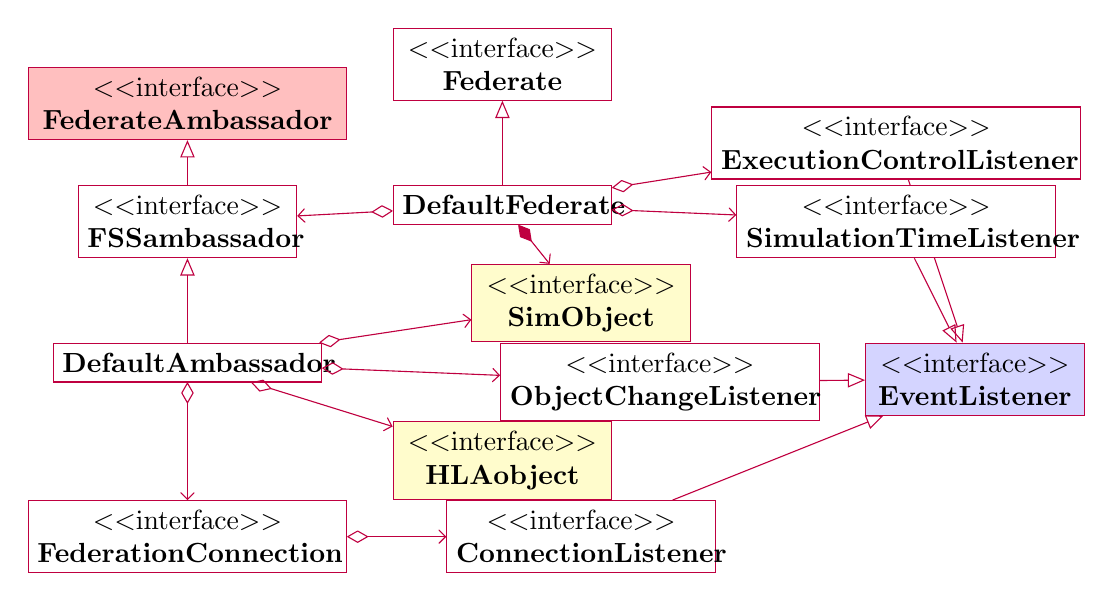
\begin{tikzpicture}% [ show background grid ]
\begin{interface}[text width=1in]{HLAobject}{0,-5}
\end{interface}

\begin{interface}[text width=1in]{SimObject}{1,-3}
\end{interface}

\begin{interface}[text width=1in,fill={rgb:blue,1;white,5}]{EventListener}{6,-4}
\end{interface}

\begin{interface}[text width=1.75in,fill=white]{ExecutionControlListener}{5,-1}
\inherit{EventListener}
\end{interface}

\begin{interface}[text width=1.5in,fill=white]{SimulationTimeListener}{5,-2}
\inherit{EventListener}
\end{interface}

\begin{interface}[text width=1.5in,fill=white]{ObjectChangeListener}{2,-4}
\inherit{EventListener}
\end{interface}

\begin{interface}[text width=1.5in,fill=pink]{FederateAmbassador}{-4,-.5}
\end{interface}

\begin{interface}[text width=1in,fill=white]{FSSambassador}{-4,-2}
\inherit{FederateAmbassador}
\end{interface}

\begin{interface}[text width=1.25in,fill=white]{ConnectionListener}{1,-6}
\inherit{EventListener}
\end{interface}

\begin{interface}[text width=1.5in,fill=white]{FederationConnection}{-4,-6}
\end{interface}
\aggregation{FederationConnection}{}{}{ConnectionListener}

\begin{class}[text width=1.25in,fill=white]{DefaultAmbassador}{-4,-4}
\inherit{FSSambassador}
\end{class}
\aggregation{DefaultAmbassador}{}{}{SimObject}
\aggregation{DefaultAmbassador}{}{}{HLAobject}
\aggregation{DefaultAmbassador}{}{}{ObjectChangeListener}
\aggregation{DefaultAmbassador}{}{}{FederationConnection}

\begin{interface}[text width=1in,fill=white]{Federate}{0,0}
\end{interface}

\begin{class}[text width=1in,fill=white]{DefaultFederate}{0,-2}
\inherit{Federate}
\end{class}
\aggregation{DefaultFederate}{}{}{FSSambassador}
\composition{DefaultFederate}{}{}{SimObject}
\aggregation{DefaultFederate}{}{}{ExecutionControlListener}
\aggregation{DefaultFederate}{}{}{SimulationTimeListener}

\end{tikzpicture}
\caption{Object class diagram of the FSS simulation toolkit HLA model implementations}
\label{fig:toolkitExecutionOCD}
\end{figure}

\subsection{Toolkit Examples}

The toolkit includes six example federates based on the case study in \textcite{grogan13}. Each federate includes a graphical user interface (GUI) for user interaction using common GUI components within the \texttt{edu.mit.fss.examples.gui} package. Five federates for FSS member simulation use customized data models within the \texttt{edu.mit.fss.examples.member} package and specialized GUI components within the \texttt{edu.mit.fss.examples.member.gui} package. A visualization federate uses the NASA World Wind application and specialized GUI components within the \texttt{edu.mit.fss.examples.visual.gui} package.

\dirtree{%
.1 trunk/.
.2 src/.
.3 edu.mit.fss.examples.
.4 CosmoSkyMed1.java\DTcomment{CosmoSkyMED-1 FSS member federate example}.
.4 ISSNode.java\DTcomment{ISS-Node FSS member federate example}.
.4 SaudiComSat.java\DTcomment{SaudiComSat FSS member federate example}.
.4 TDRSS.java\DTcomment{TDRSS FSS member federate example}.
.4 TerraSarX.java\DTcomment{TerraSAR-X FSS member federate example}.
.4 Visualization.java\DTcomment{Visualization federate example}.
.3 edu.mit.fss.examples.gui\DTcomment{Common GUI components for the examples}.
.3 edu.mit.fss.examples.member\DTcomment{Model components for the FSS member example}.
.3 edu.mit.fss.examples.member.gui\DTcomment{GUI components for the FSS member example}.
.3 edu.mit.fss.examples.visual.gui\DTcomment{GUI components for the visualization example}.
.2 data.tle\DTcomment{Two line element data for example spacecraft}.
}

\begin{figure}[p]
\centering
\includegraphics[width=4in]{cosmosScreenCapture}
\caption{Screen capture of the CosmosSkyMED-1 example federate. The top component is an \texttt{ExecutionControlPanel}, below is a \texttt{SpaceSystemPanel} with tabs for an \texttt{OrbitalElementPanel}, \texttt{PowerSubsystemPanel}, and \texttt{CommSubsystemPanel}.}
\label{fig:cosmosScreenCapture}
\end{figure}

\begin{figure}[p]
\centering
\includegraphics[width=4in]{visualizationScreenCapture}
\caption{Screen capture of the example visualization federate. The top component is an \texttt{ExecutionControlPanel}, below is a \texttt{WorldWindVisualization}.}
\label{fig:visualizationScreenCapture}
\end{figure}

\subsection{Toolkit Tutorials}

The toolkit includes four short tutorials to introduce the approach for developing federates

\dirtree{%
.1 trunk/.
.2 src/.
.3 edu.mit.fss.tutorial.part1.
.4 ClockFederate.java\DTcomment{An example federate to simulate a clock object}.
.4 TrivialClock.java\DTcomment{A simple simulation object to keep track of time}.
.3 edu.mit.fss.tutorial.part2.
.4 MobileElement.java\DTcomment{A simple \texttt{SurfaceElement} implementation}.
.4 OfflineTutorialFederate.java\DTcomment{An example federate to simulate a mobile element}.
.3 edu.mit.fss.tutorial.part3.
.4 Element1.java\DTcomment{Runs a federate for the ``Element 1'' mobile element}.
.4 Element2.java\DTcomment{Runs a federate for the ``Element 2'' mobile element}.
.4 OnlineTutorialFederate.java\DTcomment{An example federate to simulate a mobile element}.
.3 edu.mit.fss.tutorial.part4.
.4 ControlPanel.java\DTcomment{A component to display and control a mobile element}.
.4 ElementGUI.java\DTcomment{Runs a federate for a mobile element with a GUI}.
}

\subsection{Third Party Libraries}

The following third party libraries provide functionality for the toolkit:
\dirtree{%
.1 trunk/.
.2 lib/.
.3 commons-math3-3.2/\DTcomment{Apache Commons Math 3 (Orekit dependency)}.
.3 jfreechart-1.0.17/\DTcomment{JFreeChart and JCommon for user interface charts}.
.3 log4j-1.2.17/\DTcomment{Java debugging and error logging}.
.3 ohla-0.6/\DTcomment{Open HLA runtime infrastructure}.
.3 orekit-6.0/\DTcomment{Orekit spacecraft flight dynamics}.
.3 portico-2.0.0/\DTcomment{Portico HLA runtime infrastructure}.
.3 worldwind-2.0-857.1737/\DTcomment{World Wind for Earth visualization}.
.2 lib-external/.
.3 gdal/\DTcomment{Geospatial Data Abstraction Library (World Wind dependency)}.
.2 ohla-crc.properties\DTcomment{Configuration properties for OHLA central RTI component}.
.2 ohla-lrc.properties\DTcomment{Configuration properties for OHLA local RTI component}.
.2 orekit-data.zip\DTcomment{Orekit default physical data package}.
.2 RTI.rid\DTcomment{Portico RTI Initialization Data (RID) file}.
}

These libraries include two HLA runtime infrastructure (RTI) implementations. The Portico library uses UDP multicast communication which only works on local area networks. Additional configuration settings for Portico are contained within the \texttt{RTI.rid} file. The OHLA library uses TCP communication which is generally allowed over wide area networks. Additional configuration settings for OHLA are contained within the \texttt{ohla-crc.properties} and \texttt{ohla-lrc.properties} files.

The Orekit spacecraft flight dynamics library is used to define reference frames and to perform orbital propagation within the example federates. It requires a physical data package for which this toolkit uses the default file, \texttt{orekit-data.zip}.

The JFreeChart library is used within the example federates for charting and plotting capabilities.

The World Wind version distributed in this toolkit is a nightly-build dating to October 2013. It should be replaced with version 2.0 when officially released.

\section{Quick Start Tutorials}

This quick start tutorial develops new federates from the core FSS interfaces. It is intended to illustrate the concepts used to implement the example federates in the previous section through several successive parts.

Part 1 demonstrates how new objects can be defined and used in a time-stepped simulation. It implements a trivial clock simulation object and uses it to track time advancement in an offline simulation.

Part 2 demonstrates how the FSS core interfaces can be used to create a custom FSS object. It implements a mobile surface element with controllable velocity and uses it in an offline simulation.

Part 3 demonstrates an online distributed simulation using two instances of the mobile surface element implementation from Part 2. Two federates join a federated simulation and output computed distances from each other's element.

Part 4 develops a graphical user interface (GUI) to control the mobile surface elements from Part 3. The GUI allows velocity to be changed during a simulation using arrow key bindings.

Finally, Part 5 shows how to switch between using the Portico and OHLA RTI implementations.

\subsection{Part 1: Implementing a Simulation Object}

The first tutorial focuses on defining a very simple simulation object---a clock which only keeps track of time---and using it in an offline simulation. First, we define the \texttt{TrivialClock} object class implementing the \texttt{SimObject} interface described in Box \ref{lst:trivialClock}. It contains data members for its name and time, and a temporary variable to hold the next time between \texttt{tick} and \texttt{tock} method calls. We also include a \texttt{getDate()} method to convert the integer-based time in milliseconds to a Java \texttt{Date} object.

\begin{Code}
\begin{lstlisting}[caption={TrivialClock object class},label={lst:trivialClock}]
package edu.mit.fss.tutorial.part1;

import java.util.ArrayList;
import java.util.Collection;
import java.util.Date;
import edu.mit.fss.SimObject;

public class TrivialClock implements SimObject {
	private String name;
	private long time, nextTime;
	
	public TrivialClock(String name) {
		this.name = name;
	}
	public Date getDate() {
		return new Date(time);
	}
	public String getName() {
		return name;
	}
	public Collection<? extends SimObject> getNestedObjects() {
		return new ArrayList<SimObject>();
	}
	public long getTime() {
		return time;
	}
	public void initialize(long time) {
		this.time = time;
	}
	public void tick(long duration) {
		nextTime = time + duration;
	}
	public void tock() {
		time = nextTime;
	}
}
\end{lstlisting}
\end{Code}

Next we define a new federate to use a \texttt{TrivialClock} object instance. The \texttt{ClockFederate} object class in Box \ref{lst:clockFederate} trivially extends the \texttt{DefaultFederate} class. Its main method runs the federate, performing the following actions:
\begin{enumerate}
\item Configures log messages.
\item Instantiates a new trivial clock object instance (\texttt{clock}).
\item Instantiates a new clock federate instance (\texttt{fed}).
\item Adds the clock instance to the federate.
\item Adds a \texttt{SimulationTimeListener} to the federate to log messages whenever the simulation time advances.
\item Sets the federate's initial (0 s) and final (20 s) times and the time step (1 s).
\item Configures the federate to execute in offline mode.
\item Initializes, runs, and finally exist the federate.
\end{enumerate}

\begin{Code}
\begin{lstlisting}[caption={ClockFederate object class},label={lst:clockFederate}]
package edu.mit.fss.tutorial.part1;

import hla.rti1516e.exceptions.RTIexception;
import org.apache.log4j.BasicConfigurator;
import org.apache.log4j.Level;
import org.apache.log4j.Logger;
import edu.mit.fss.DefaultFederate;
import edu.mit.fss.event.SimulationTimeEvent;
import edu.mit.fss.event.SimulationTimeListener;

public class ClockFederate extends DefaultFederate {
	private static Logger logger = Logger.getLogger("edu.mit.fss");

	public ClockFederate() throws RTIexception {
		super();
	}
	public static void main(String[] args) throws RTIexception {
		BasicConfigurator.configure();
		logger.setLevel(Level.INFO);
		
		final TrivialClock clock = new TrivialClock("My clock");
		
		ClockFederate fed = new ClockFederate();
		fed.addObject(clock);
		fed.addSimulationTimeListener(new SimulationTimeListener() {
			public void timeAdvanced(SimulationTimeEvent event) {
				logger.info("The clock reads " + clock.getDate() + ".");
			}
		});
		fed.setInitialTime(0);
		fed.setFinalTime(20000);
		fed.setTimeStep(1000);
		fed.getConnection().setOfflineMode(true);
		fed.initialize();
		fed.run();
		fed.exit();
	}
}
\end{lstlisting}
\end{Code}

A sample output from running the main method in \texttt{ClockFederate} is displayed in Box \ref{lst:part1Output}. The numbers on the left show the system time (in milliseconds) and the bracketed term identifies the thread executing the log comment (the main thread in this case). The default minimum step duration is quite visible in this case as each simulation time step is throttled to take at least 100 ms.

\begin{Code}
\begin{lstlisting}[caption={ClockFederate main output},label={lst:part1Output},numbers=none]
239 [main] INFO edu.mit.fss  - The clock reads Wed Dec 31 19:00:00 EST 1969.
243 [main] INFO edu.mit.fss  - The clock reads Wed Dec 31 19:00:01 EST 1969.
355 [main] INFO edu.mit.fss  - The clock reads Wed Dec 31 19:00:02 EST 1969.
455 [main] INFO edu.mit.fss  - The clock reads Wed Dec 31 19:00:03 EST 1969.
555 [main] INFO edu.mit.fss  - The clock reads Wed Dec 31 19:00:04 EST 1969.
655 [main] INFO edu.mit.fss  - The clock reads Wed Dec 31 19:00:05 EST 1969.
755 [main] INFO edu.mit.fss  - The clock reads Wed Dec 31 19:00:06 EST 1969.
855 [main] INFO edu.mit.fss  - The clock reads Wed Dec 31 19:00:07 EST 1969.
955 [main] INFO edu.mit.fss  - The clock reads Wed Dec 31 19:00:08 EST 1969.
1055 [main] INFO edu.mit.fss  - The clock reads Wed Dec 31 19:00:09 EST 1969.
1155 [main] INFO edu.mit.fss  - The clock reads Wed Dec 31 19:00:10 EST 1969.
1255 [main] INFO edu.mit.fss  - The clock reads Wed Dec 31 19:00:11 EST 1969.
1355 [main] INFO edu.mit.fss  - The clock reads Wed Dec 31 19:00:12 EST 1969.
1455 [main] INFO edu.mit.fss  - The clock reads Wed Dec 31 19:00:13 EST 1969.
1555 [main] INFO edu.mit.fss  - The clock reads Wed Dec 31 19:00:14 EST 1969.
1655 [main] INFO edu.mit.fss  - The clock reads Wed Dec 31 19:00:15 EST 1969.
1755 [main] INFO edu.mit.fss  - The clock reads Wed Dec 31 19:00:16 EST 1969.
1856 [main] INFO edu.mit.fss  - The clock reads Wed Dec 31 19:00:17 EST 1969.
1955 [main] INFO edu.mit.fss  - The clock reads Wed Dec 31 19:00:18 EST 1969.
2055 [main] INFO edu.mit.fss  - The clock reads Wed Dec 31 19:00:19 EST 1969.
2155 [main] INFO edu.mit.fss  - The clock reads Wed Dec 31 19:00:20 EST 1969.
\end{lstlisting}
\end{Code}

\subsection{Part 2: Implementing an FSS Element}

The second part of this tutorial implements an FSS element capable of participating in a federated simulation. For simplicity, we implement a \texttt{SurfaceElement} relying on a basic Earth-fixed Cartesian coordinate system (XY-plane on the equator, positive-X towards the prime meridian, positive-Y towards 90-degrees longitude, and positive-Z towards the North pole). 

Box \ref{lst:mobileElement} describes the implementation of the \texttt{MobileElement} object class. It includes data members for its name, position, and velocity with additional data members to temporarily store the next and initial positions and velocities. The constructor takes a name and initial velocity as arguments and sets other variables to default values.

The \texttt{tick} method uses a simple Euler integration to propagate position based on an assumption of fixed velocity. A more sophisticated implementation may use a higher-fidelity integrator such as one from a selection of Runge-Kutta integrators included in the Apache Commons Math library.

The Geodetic coordinate implementations (i.e. latitude, longitude, and altitude) use an inaccurate spherical Earth model, i.e. they are computed using simple spherical coordinate transforms assuming a constant radius of 6371 kilometers rather than the standard WGS84 Earth model assumed for the ITRF2008 reference frame. The toolkit-provided \texttt{OrekitSurfaceElement}, for example, uses the WGS84 model parameters in the Orekit library to transform between Cartesian and Geodetic coordinates.

\begin{Code}
\begin{lstlisting}[caption={MobileElement object class},label={lst:mobileElement}]
package edu.mit.fss.tutorial.part2;

import java.util.ArrayList;
import java.util.Collection;
import org.apache.commons.math3.geometry.euclidean.threed.Vector3D;
import edu.mit.fss.ReferenceFrame;
import edu.mit.fss.SimObject;
import edu.mit.fss.SurfaceElement;

public class MobileElement implements SurfaceElement {
	private String name;
	private Vector3D position, nextPosition, initialPosition;
	private Vector3D velocity, nextVelocity, initialVelocity;
	
	public MobileElement(String name, Vector3D initialVelocity) {
		this.name = name;
		position = new Vector3D(0, 0, 0);
		initialPosition = new Vector3D(0, 0, 0);
		velocity = new Vector3D(0, 0, 0);
		this.initialVelocity = initialVelocity;
	}
	public double getAltitude() { return position.getNorm() - 6371e3; }
	public ReferenceFrame getFrame() { return ReferenceFrame.ITRF2008; }
	public double getLatitude() {
		return Math.toDegrees(Math.atan2(position.getZ(), position.getX()));
	}
	public double getLongitude() {
		return Math.toDegrees(Math.atan2(position.getY(), position.getX()));
	}
	public String getName() { return name; }
	public Collection<? extends SimObject> getNestedObjects() {
		return new ArrayList<SimObject>();
	}
	public Vector3D getPosition() { return position; }
	public Vector3D getVelocity() { return velocity; }
	public void initialize(long time) {
		position = initialPosition;
		nextPosition = initialPosition;
		velocity = initialVelocity;
		nextVelocity = initialVelocity;
	}
	public void setVelocity(Vector3D velocity) { nextVelocity = velocity; }
	public void tick(long duration) {
		nextPosition = position.add(velocity.scalarMultiply(duration/1000d));
	}
	public void tock() {
		position = nextPosition;
		velocity = nextVelocity;
	}
}
\end{lstlisting}
\end{Code}

We will use the \texttt{MobileElement} implementation throughout the rest of the tutorial exercises. First, however, let's test in an offline federation. Box \ref{lst:offlineTutorialFederate} extends the federate developed in Part 1 to include a new mobile element. Note that as it is initialized to the center of the Earth (0,0,0), there is no physical interpretation for this particular element.

\begin{Code}
\begin{lstlisting}[caption={OfflineTutorialFederate object class},label={lst:offlineTutorialFederate}]
package edu.mit.fss.tutorial.part2;

import hla.rti1516e.exceptions.RTIexception;
import org.apache.commons.math3.geometry.euclidean.threed.Vector3D;
import org.apache.log4j.BasicConfigurator;
import org.apache.log4j.Level;
import org.apache.log4j.Logger;
import edu.mit.fss.DefaultFederate;
import edu.mit.fss.event.SimulationTimeEvent;
import edu.mit.fss.event.SimulationTimeListener;

public class OfflineTutorialFederate extends DefaultFederate {
	private static Logger logger = Logger.getLogger("edu.mit.fss");

	public OfflineTutorialFederate(final MobileElement element) throws RTIexception {
		super();
		addObject(element);
		addSimulationTimeListener(new SimulationTimeListener() {
			public void timeAdvanced(SimulationTimeEvent event) {
				logger.info("At time " + event.getTime() + ", " 
						+ element.getName() + " is at " 
						+ element.getPosition() + ".");
			}
		});
	}
	public void execute(long initialTime, long finalTime, long timeStep) {
		setInitialTime(initialTime);
		setFinalTime(finalTime);
		setTimeStep(timeStep);
		getConnection().setOfflineMode(true);
		initialize();
		run();
	}
	public static void main(String[] args) throws RTIexception {
		BasicConfigurator.configure();
		logger.setLevel(Level.INFO);
		MobileElement element = new MobileElement("Element", new Vector3D(10, 0, 0));
		OfflineTutorialFederate fed = new OfflineTutorialFederate(element);
		fed.execute(0, 20000, 1000);
		fed.exit();
	}
}
\end{lstlisting}
\end{Code}

The \texttt{OfflineTutorialFederate} includes more internal structure than \texttt{ClockFederate}. In particular, several instructions have been moved to the constructor and others to a new \texttt{execute} method. The constructor adds the mobile element to the federate and adds a \texttt{SimulationTimeListener} to log messages during the simulation execution. The \texttt{execute} method sets the initial and final time, the time step, configures the federate for offline simulation, and initializes and runs the federate.

The main method contains other instructions, such as configuring logging, specifying the mobile element object instantiation (with initial velocity of 10 m/s in the X-direction) and federate object instantiation. It also defines the execution period between 0 and 20 seconds with a 1-second time step. After the federate executes, it exits.

Box \ref{lst:part2Output} displays a sample output from the main method. The element moves 10 meters in the x-direction during each 1-second time step according to its constant velocity.

\begin{Code}
\begin{lstlisting}[caption={OfflineTutorialFederate main output},label={lst:part2Output},numbers=none]
218 [main] INFO edu.mit.fss  - At time 0, Element is at {0; 0; 0}.
221 [main] INFO edu.mit.fss  - At time 1000, Element is at {10; 0; 0}.
330 [main] INFO edu.mit.fss  - At time 2000, Element is at {20; 0; 0}.
430 [main] INFO edu.mit.fss  - At time 3000, Element is at {30; 0; 0}.
530 [main] INFO edu.mit.fss  - At time 4000, Element is at {40; 0; 0}.
630 [main] INFO edu.mit.fss  - At time 5000, Element is at {50; 0; 0}.
730 [main] INFO edu.mit.fss  - At time 6000, Element is at {60; 0; 0}.
830 [main] INFO edu.mit.fss  - At time 7000, Element is at {70; 0; 0}.
943 [main] INFO edu.mit.fss  - At time 8000, Element is at {80; 0; 0}.
1043 [main] INFO edu.mit.fss  - At time 9000, Element is at {90; 0; 0}.
1143 [main] INFO edu.mit.fss  - At time 10000, Element is at {100; 0; 0}.
1243 [main] INFO edu.mit.fss  - At time 11000, Element is at {110; 0; 0}.
1343 [main] INFO edu.mit.fss  - At time 12000, Element is at {120; 0; 0}.
1444 [main] INFO edu.mit.fss  - At time 13000, Element is at {130; 0; 0}.
1543 [main] INFO edu.mit.fss  - At time 14000, Element is at {140; 0; 0}.
1643 [main] INFO edu.mit.fss  - At time 15000, Element is at {150; 0; 0}.
1743 [main] INFO edu.mit.fss  - At time 16000, Element is at {160; 0; 0}.
1843 [main] INFO edu.mit.fss  - At time 17000, Element is at {170; 0; 0}.
1944 [main] INFO edu.mit.fss  - At time 18000, Element is at {180; 0; 0}.
2043 [main] INFO edu.mit.fss  - At time 19000, Element is at {190; 0; 0}.
2143 [main] INFO edu.mit.fss  - At time 20000, Element is at {200; 0; 0}.
\end{lstlisting}
\end{Code}

\subsection{Part 3: Running a Federated Simulation}

The third part of this tutorial uses the \texttt{MobileElement} object developed in Part 2 in an online federated simulation. Box \ref{lst:onlineTutorialFederate} implements the \texttt{OnlineTutorialFederate} as an extension of the offline federate developed in Part 2 with several additions. 

First, two new data members, \texttt{thisElement} and \texttt{otherElements} are added to track the local and remote objects respectively. The \texttt{otherElements} object uses a synchronized list for thread safety as the HLA uses a separate thread for object updates. The constructor adds a synchronized loop to print information for the \texttt{otherElements} within the \texttt{SimulationTimeListener} and adds an \texttt{ObjectChangeListener} to add or remove objects from the \texttt{otherElements} list. Finally, the \texttt{execute} method configures the federate name, type, federation name, and FOM path.

\begin{Code}
\begin{lstlisting}[caption={OnlineTutorialFederate object class},label={lst:onlineTutorialFederate}]
package edu.mit.fss.tutorial.part3;
import hla.rti1516e.exceptions.RTIexception;
import java.util.ArrayList;
import java.util.Collections;
import java.util.List;
import org.apache.log4j.Logger;
import edu.mit.fss.DefaultFederate;
import edu.mit.fss.SurfaceElement;
import edu.mit.fss.event.*;
import edu.mit.fss.tutorial.part2.MobileElement;
public class OnlineTutorialFederate extends DefaultFederate {
	private static Logger logger = Logger.getLogger(OnlineTutorialFederate.class);
	private MobileElement thisElement;
	private List<SurfaceElement> otherElements = Collections.synchronizedList(
				new ArrayList<SurfaceElement>());
	public OnlineTutorialFederate(MobileElement element) throws RTIexception {
		super();
		thisElement = element; addObject(element);
		addSimulationTimeListener(new SimulationTimeListener() {
			public void timeAdvanced(SimulationTimeEvent event) {
				logger.info("At time " + event.getTime() + ", " + thisElement.getName() 
						+ " is at " + thisElement.getPosition() + ".");
				synchronized(otherElements) {
					for(SurfaceElement e : otherElements) {
						logger.info("... distance to " + e.getName() + " is " 
								+ thisElement.getPosition().distance(e.getPosition()) + ".");
					}
				}
			}
		});
		addObjectChangeListener(new ObjectChangeListener() {
			public void objectDiscovered(ObjectChangeEvent event) {
				if(event.getObject() instanceof SurfaceElement
						&& event.getObject() != thisElement) {
					otherElements.add((SurfaceElement) event.getObject());
				}
			}
			public void objectRemoved(ObjectChangeEvent event) { 
				otherElements.remove(event.getObject());
			}
			public void objectChanged(ObjectChangeEvent event) { 	}
			public void interactionOccurred(ObjectChangeEvent event) { 	}
		});
	}
	public void execute(long initialTime, long finalTime, long timeStep) {
		setInitialTime(initialTime); setFinalTime(finalTime); setTimeStep(timeStep);
		getConnection().setOfflineMode(false);
		getConnection().setFederateName(thisElement.getName());
		getConnection().setFederateType("Demo");
		getConnection().setFederationName("Tutorial");
		getConnection().setFomPath("fss.xml");
		connect(); initialize(); run();
	}
}
\end{lstlisting}
\end{Code}

Boxes \ref{lst:element1} and \ref{lst:element2} create main methods for two federates. They use a similar form with differences in element name (Element 1 and Element 2) and initial velocity (-10 m/s in the X-direction and +5 m/s in the Y-direction).

\begin{Code}
\begin{lstlisting}[caption={Element1 object class},label={lst:element1}]
package edu.mit.fss.tutorial.part3;

import hla.rti1516e.exceptions.RTIexception;
import org.apache.commons.math3.geometry.euclidean.threed.Vector3D;
import org.apache.log4j.BasicConfigurator;
import org.apache.log4j.Level;
import org.apache.log4j.Logger;
import edu.mit.fss.tutorial.part2.MobileElement;

public abstract class Element1 {
	private static Logger logger = Logger.getLogger("edu.mit.fss");

	public static void main(String[] args) throws RTIexception {
		BasicConfigurator.configure();
		logger.setLevel(Level.INFO);
		
		MobileElement element = new MobileElement("Element 1", new Vector3D(10, 0, 0));
		OnlineTutorialFederate fed = new OnlineTutorialFederate(element);
		fed.execute(0, 50000, 1000);
		fed.exit();
	}
}
\end{lstlisting}
\end{Code}

\begin{Code}
\begin{lstlisting}[caption={Element2 object class},label={lst:element2}]
package edu.mit.fss.tutorial.part3;

import hla.rti1516e.exceptions.RTIexception;
import org.apache.commons.math3.geometry.euclidean.threed.Vector3D;
import org.apache.log4j.BasicConfigurator;
import org.apache.log4j.Level;
import org.apache.log4j.Logger;
import edu.mit.fss.tutorial.part2.MobileElement;

public abstract class Element2 {
	private static Logger logger = Logger.getLogger("edu.mit.fss");

	public static void main(String[] args) throws RTIexception {
		BasicConfigurator.configure();
		logger.setLevel(Level.INFO);
		
		MobileElement element = new MobileElement("Element 2", new Vector3D(0, 5, 0));
		OnlineTutorialFederate fed = new OnlineTutorialFederate(element);
		fed.execute(0, 50000, 1000);
		fed.exit();
	}
}
\end{lstlisting}
\end{Code}

Boxes \ref{lst:part3Output1} and \ref{lst:part3Output2} illustrate output from the two federates. In this particular case, the Element1 federate starts first and the Element2 federate joins the federation at simulation time 15000. Note the differences between the main thread (\texttt{[main]}) and the other thread (\texttt{[Thread-0]}) in logging statements. Also note the relative delay in updating element attributes: the Element2 name is not received by Element1 until 16000 and the Element1 name is not received by Element2 until 17000. The timing of all of these events is dependent on network latency, processor utilization, and other operating system factors not easily controllable without additional HLA services such as synchronization points.

\begin{Code}
\begin{lstlisting}[caption={Element1 partial main output},label={lst:part3Output1},numbers=none]
13674 [Thread-0] INFO edu.mit.fss...  - Time advance granted to logical time 13000.0
13675 [main] INFO edu.mit.fss...  - At time 13000, Element 1 is at {130; 0; 0}.
13788 [Thread-0] INFO edu.mit.fss...  - Time advance granted to logical time 14000.0
13788 [main] INFO edu.mit.fss...  - At time 14000, Element 1 is at {140; 0; 0}.
13851 [Thread-0] INFO edu.mit.fss...  - Time advance granted to logical time 15000.0
13851 [main] INFO edu.mit.fss...  - At time 15000, Element 1 is at {150; 0; 0}.
15080 [Thread-0] INFO edu.mit.fss...  - Discovering object instance 2097153.
15095 [Thread-0] INFO edu.mit.fss...  - Time advance granted to logical time 16000.0
15095 [main] INFO edu.mit.fss... - At time 16000, Element 1 is at {160; 0; 0}.
15095 [main] INFO edu.mit.fss...  - ... distance to Element 2 is 160.0781059358212.
15158 [Thread-0] INFO edu.mit.fss...  - Time advance granted to logical time 17000.0
15158 [main] INFO edu.mit.fss...  - At time 17000, Element 1 is at {170; 0; 0}.
15159 [main] INFO edu.mit.fss...  - ... distance to Element 2 is 170.29386365926402.
\end{lstlisting}
\end{Code}

\begin{Code}
\begin{lstlisting}[caption={Element2 partial main output},label={lst:part3Output2},numbers=none]
10232 [main] INFO edu.mit.fss...  - Joined federation execution Tutorial as federate Element 2 of type Demo.
10240 [main] INFO edu.mit.fss...  - Asynchronous message delivery enabled.
10247 [Thread-0] INFO edu.mit.fss...  - Time constrained enabled with logical time 0.0.
10247 [main] INFO edu.mit.fss...  - Time constrained behavior enabled.
10251 [Thread-0] INFO edu.mit.fss...  - Time regulation enabled with logical time 15000.0.
11250 [main] INFO edu.mit.fss...  - Time regulating behavior enabled.
11270 [Thread-0] INFO edu.mit.fss...  - Discovering object instance 2.
11378 [main] INFO edu.mit.fss...  - Published and subscribed all objects and interactions.
11384 [main] INFO edu.mit.fss...  - At time 15000, Element 2 is at {0; 0; 0}.
11396 [main] INFO edu.mit.fss...  - ... distance to  is 0.0.
11426 [Thread-0] INFO edu.mit.fss...  - Time advance granted to logical time 16000.0
11426 [main] INFO edu.mit.fss...  - At time 16000, Element 2 is at {0; 5; 0}.
11426 [main] INFO edu.mit.fss...  - ... distance to  is 5.0.
11503 [Thread-0] INFO edu.mit.fss...  - Time advance granted to logical time 17000.0
11505 [main] INFO edu.mit.fss...  - At time 17000, Element 2 is at {0; 10; 0}.
11506 [main] INFO edu.mit.fss...  - ... distance to Element 1 is 170.29386365926402.
\end{lstlisting}
\end{Code}

\subsection{Part 4: Creating a Graphical User Interface}

The fourth part of this tutorial builds a graphical user interface to control a \texttt{MobileElement} object as a federate. Boxes \ref{lst:controlPanel1} and \ref{lst:controlPanel2} develop a \texttt{ControlPanel} object class which displays the spatial state of a federate in a graphical user interface.

Similar to the \texttt{OnlineTutorialFederate}, it contains data members \texttt{boundElement} and \texttt{elements} for a local element and list of remote elements (again using a synchronized list). A \texttt{KeyAdapter} object added in the constructor responds to key presses to control the velocity of the bound element. Methods from the \texttt{ObjectChangeListener} interface add or remove elements or prompt a repainting of the display. Finally, the \texttt{paint} method uses a custom method to update the display, using lines for x- and y-axes and circles (with labels) for each element. The bound element is drawn in blue while other elements are drawn in black.

\begin{Code}
\begin{lstlisting}[caption={ControlPanel object class},label={lst:controlPanel1}]
package edu.mit.fss.tutorial.part4;

import java.awt.Color;
import java.awt.Dimension;
import java.awt.Graphics;
import java.awt.event.KeyAdapter;
import java.awt.event.KeyEvent;
import java.util.ArrayList;
import java.util.Collections;
import java.util.List;
import javax.swing.JPanel;
import org.apache.commons.math3.geometry.euclidean.threed.Vector3D;
import edu.mit.fss.SurfaceElement;
import edu.mit.fss.event.ObjectChangeEvent;
import edu.mit.fss.event.ObjectChangeListener;
import edu.mit.fss.tutorial.part2.MobileElement;

public class ControlPanel extends JPanel implements ObjectChangeListener {
	private static final long serialVersionUID = -1729012305362962099L;
	private static float DISPLAY_SCALE = 5.0f;
	private static int ELEMENT_SIZE = 4;
	private MobileElement boundElement;
	private List<SurfaceElement> elements = Collections.synchronizedList(new ArrayList<SurfaceElement>());
	public ControlPanel() {
		setFocusable(true);
		setPreferredSize(new Dimension(300,300));
		setBackground(Color.white);
		addKeyListener(new KeyAdapter() {
			public void keyPressed(KeyEvent e) {
				if(boundElement==null) { return; }
				if(e.getKeyCode()==KeyEvent.VK_UP) {
					boundElement.setVelocity(boundElement.getVelocity().add(new Vector3D(0,1,0)));
				} else if(e.getKeyCode()==KeyEvent.VK_DOWN) {
					boundElement.setVelocity(boundElement.getVelocity().add(new Vector3D(0,-1,0)));
				} else if(e.getKeyCode()==KeyEvent.VK_LEFT) {
					boundElement.setVelocity(boundElement.getVelocity().add(new Vector3D(-1,0,0)));
				} else if(e.getKeyCode()==KeyEvent.VK_RIGHT) {
					boundElement.setVelocity(boundElement.getVelocity().add(new Vector3D(1,0,0)));
				}
			}
		});
	}
	private int[] getScreenLocation(Vector3D position) {
		int x = (int) Math.round(getWidth()/2 + position.getX()/DISPLAY_SCALE);
		int y = (int) Math.round(getHeight()/2 - position.getY()/DISPLAY_SCALE);
		return new int[]{x, y};
	}
	public void interactionOccurred(ObjectChangeEvent event) { }
\end{lstlisting}
\end{Code}

\begin{Code}
\begin{lstlisting}[caption={ControlPanel object class (continued)},label={lst:controlPanel2}]
	public void objectChanged(ObjectChangeEvent event) { 
		repaint(); 
	}
	public void objectDiscovered(ObjectChangeEvent event) {
		if(event.getObject() instanceof SurfaceElement) {
			elements.add((SurfaceElement) event.getObject());
		}
	}
	public void objectRemoved(ObjectChangeEvent event) {
		elements.remove(event.getObject());
	}
	public void paint(Graphics g) {
		super.paint(g);
		g.setColor(Color.gray);
		g.drawLine(0, getHeight()/2, getWidth(), getHeight()/2);
		g.drawLine(getWidth()/2, 0, getWidth()/2, getHeight());
		synchronized(elements) {
			for(SurfaceElement e : elements) {
				if(e instanceof MobileElement) {
					g.setColor(Color.blue);
				} else {
					g.setColor(Color.black);
				}
				int[] location = getScreenLocation(e.getPosition());
				g.fillOval(location[0] - ELEMENT_SIZE/2, 
						location[1] - ELEMENT_SIZE/2, 
						ELEMENT_SIZE, ELEMENT_SIZE);
				g.drawString(e.getName(), location[0] + ELEMENT_SIZE/2 + 2, 
						location[1] + ELEMENT_SIZE/2 + ELEMENT_SIZE/2);
			}
		}
	}
	public void setBoundElement(MobileElement element) {
		this.boundElement = element;
	}
}
\end{lstlisting}
\end{Code}

Box \ref{lst:elementGUI} develops the \texttt{ElementGUI} class which holds the main method to run the federate. It uses a \texttt{JOptionPane} to allow user input for a name of the local mobile element instance. Finally it creates a \texttt{ControlPanel} object instance, adds it as an \texttt{ObjectChangeListener} to an \texttt{OnlineTutorialFederate}, and launches the GUI in a \texttt{JFrame}.

\begin{Code}
\begin{lstlisting}[caption={ElementGUI object class},label={lst:elementGUI}]
package edu.mit.fss.tutorial.part4;

import hla.rti1516e.exceptions.RTIexception;
import java.awt.event.WindowAdapter;
import java.awt.event.WindowEvent;
import java.lang.reflect.InvocationTargetException;
import javax.swing.JFrame;
import javax.swing.JOptionPane;
import javax.swing.SwingUtilities;
import org.apache.commons.math3.geometry.euclidean.threed.Vector3D;
import org.apache.log4j.BasicConfigurator;
import org.apache.log4j.Level;
import org.apache.log4j.Logger;
import edu.mit.fss.tutorial.part2.MobileElement;
import edu.mit.fss.tutorial.part3.OnlineTutorialFederate;

public abstract class ElementGUI {
	private static Logger logger = Logger.getLogger("edu.mit.fss");
	
	public static void main(String[] args) throws RTIexception {
		BasicConfigurator.configure();
		logger.setLevel(Level.INFO);
		String name = null;
		while(name == null || name.isEmpty()) {
			name = JOptionPane.showInputDialog("Enter element name:");
		}
		final MobileElement element = new MobileElement(name, new Vector3D(0, 0, 0));
		final OnlineTutorialFederate fed = new OnlineTutorialFederate(element);
		try {
			SwingUtilities.invokeAndWait(new Runnable() {
				public void run() {
					ControlPanel controlPanel = new ControlPanel();
					controlPanel.setBoundElement(element);
					fed.addObjectChangeListener(controlPanel);
					JFrame frame = new JFrame();
					frame.setContentPane(controlPanel);
					frame.pack();
					frame.setVisible(true);
					frame.addWindowListener(new WindowAdapter() {
						public void windowClosing(WindowEvent e) {
							fed.exit();
						}
					});
				}
			});
		} catch (InvocationTargetException | InterruptedException e) {
			logger.error(e);
		}
		fed.execute(0, Long.MAX_VALUE, 1000);
	}
}
\end{lstlisting}
\end{Code}

Figure \ref{fig:elementScreenCapture} shows screen captures of two instances of a \texttt{ElementGUI}. They display both elements on the X-Y plane, using blue for the local element with velocity controllable with arrow keys and black for the remote element.

\begin{figure}
\centering
\includegraphics[width=2.5in]{element1ScreenCapture} \hspace{.125in}
\includegraphics[width=2.5in]{element2ScreenCapture}
\caption{Screen capture of two \texttt{ElementGUI} instances. Left: bound element is named ``Element 1.'' Right: bound element is named ``Element 2.''}
\label{fig:elementScreenCapture}
\end{figure}

\subsection{Part 5: Switching between Portico and OHLA RTIs}

This section describes how to switch between Portico and OHLA RTIs for a federation. While both implement the IEEE 1516-2010 standard, they do so to varying degrees which complicates switching between them. Fortunately, the major differences can be isolated to a few factors which have been built into the \texttt{DefaultAmbassador} class. Portico is the default RTI as it is slightly simpler to use. This section discusses how to change to the OHLA RTI.

\begin{enumerate}
\item Configure and start the OHLA Central RTI Component (CRC).
\begin{enumerate}
\item Configure the \texttt{ohla-crc.properties} file: choose the desired port number (default 15000).
\item Configure the firewall: add rules (if necessary) to allow inbound and outbound TCP traffic on the desired port.
\item Start the CRC program: run the main method in \texttt{edu.mit.fss.hla.OHLA\_CRC.java}.
\end{enumerate}
\item Configure the OHLA Local RTI Component (LRC).
\begin{enumerate}
\item Configure the \texttt{ohla-lrc.properties} file: select the CRC host address (IP or host name) and associated port number.
\item Configure the firewall: add rules (if necessary) to allow inbound and outbound TCP traffic on the desired port.
\end{enumerate}
\item Configure and run the federate.
\begin{enumerate}
\item Add or change the \texttt{DefaultAmbassador} constructor argument from \texttt{PORTICO\_RTI} (also the default for no arguments) to \texttt{DefaultAmbassador.OHLA\_RTI}.
\item Run the federate normally.
\end{enumerate}
\end{enumerate}

For example, the change in the ISS example federate is shown in Boxes \ref{lst:issPortico}--\ref{lst:issOHLA} as a change in its constructor.

\begin{Code}
\begin{lstlisting}[caption={ISSFederate constructor with Portico RTI},label={lst:issPortico}]
	public ISSFederate() throws RTIexception {
		super(new DefaultAmbassador(DefaultAmbassador.PORTICO_RTI));
	}
\end{lstlisting}

\begin{lstlisting}[caption={ISSFederate constructor with OHLA RTI},label={lst:issOHLA}]
	public ISSFederate() throws RTIexception {
		super(new DefaultAmbassador(DefaultAmbassador.OHLA_RTI));
	}
\end{lstlisting}
\end{Code}

Similarly, Boxes \ref{lst:tutorialPortico}--\ref{lst:tutorialOHLA} show the change in constructor for the \texttt{OnlineTutorialFederate} from Parts 3--4.

\begin{Code}
\begin{lstlisting}[caption={OnlineTutorialFederate constructor with Portico RTI},label={lst:tutorialPortico}]
	public OnlineTutorialFederate(MobileElement element) throws RTIexception {
		super();
\end{lstlisting}

\begin{lstlisting}[caption={OnlineTutorialFederate constructor with OHLA RTI},label={lst:tutorialOHLA}]
	public OnlineTutorialFederate(MobileElement element) throws RTIexception {
		super(new DefaultAmbassador(DefaultAmbassador.OHLA_RTI)));
\end{lstlisting}
\end{Code}

Some caveats:
\begin{itemize}
\item The OHLA CRC is relatively fragile and does not handle exceptions very well, such as unexpected loss-of-connection to federates. Be prepared to restart it as necessary.
\item Only one OHLA CRC can be bound to a port at a time. An exception will appear if two attempts are made.
\end{itemize}

\end{document}
